\documentclass{standalone}
\usepackage{tikz,amsmath}
\usetikzlibrary{angles,quotes}
\begin{document}
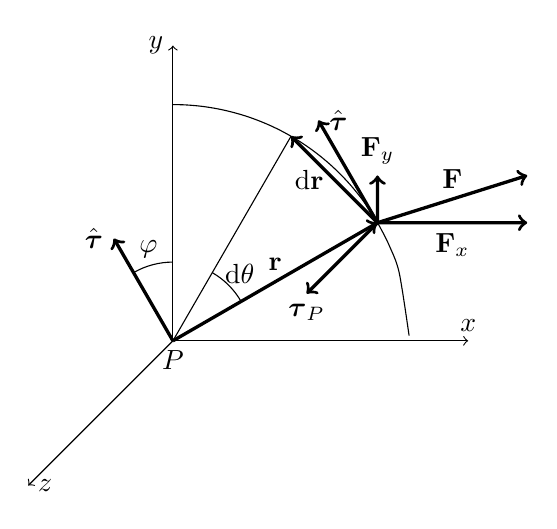
\begin{tikzpicture}[scale=3]
    \coordinate(O) at (0,0)node[below]{$P$};
    \draw[->](O)--(1.25,0)node[above]{$x$};
    \draw[->](O)--(0,1.25)coordinate(y)node[left]{$y$};
    \draw[->](O)--(-0.6125,-0.6125)node[right]{$z$};
    
    \draw[-]plot[smooth, domain=0:1](\x,{(1-(\x)^2)^0.5});

    \draw[-](O)--(0.5,0.866)coordinate(p);
    \draw[->,very thick](O)--(0.866,0.5)coordinate(a)node[midway, above]{$\mathbf{r}$};
    \draw[->,very thick](a)--(p)node[midway, left]{$\mathrm{d}\mathbf{r}$};
    \draw[->,very thick](a)--(1.5,0.7)node[midway, above]{$\mathbf{F}$};
    \draw[->,very thick](a)--(1.5,0.5)node[midway, below]{$\mathbf{F}_x$};
    \draw[->,very thick](a)--(0.866,0.7)node[above]{$\mathbf{F}_y$};
    \draw[->,very thick](a)--(0.616,0.933)node[right]{$\hat{\boldsymbol{\tau}}$};
    \draw[->,very thick](a)--(0.566,0.2)node[below]{$\boldsymbol{\tau}_P$};
    \draw[->,very thick](O)--(-0.25,0.433)coordinate(tau)node[left]{$\hat{\boldsymbol{\tau}}$};

    \pic["$\varphi$",draw, angle eccentricity=1.2, angle radius=1cm]{angle=y--O--tau};
    \pic["$\mathrm{d}\theta$",draw, angle eccentricity=1.2, angle radius=1cm]{angle=a--O--p};
\end{tikzpicture}
\end{document}